
The original issue addressed in this work is to find an appropriate method to represent emulsion or any ploy disperse multiphase flow within an averaging framework.
Indeed, due to the multiscale physical phenomenon present in those flows it is rather difficult to model the classical governing equations of fluids mechanics.  
Therefore, in this manuscript we presented a clear workflow providing accurate tools for the modeling of multiphase flows. 

The devellopement presented in this manuscript can be summaries into 9 key points:
\begin{enumerate}
    \item \ref{chap:daniel1} provides a derivation of the averaged equations governing the motion of dispersed two-phase flows with interfacial transport. 
    The averaged equations for the dispersed phase are derived through two distinct approaches: the particle-averaged (or Lagrangian) formalism, and the phase-averaged method. 
    The main conclusion of this work is the demonstration of the relation between the particle-averaged and phase-averaged equations. 
    We show that the dispersed phase-averaged equations can be interpreted as a series expansion of the particle-averaged moment equations. 
    The paper concludes by presenting a "hybrid" set of equations, consisting of phase-averaged equations for the continuous fluid phase, complemented by an arbitrary number of moment conservation equations for the dispersed phase.
    \item Following this we expose in \ref{chap:daniel15} the mass, momentum and energy averaged equations, using the ``hybrid'' formalism, that are necessary to describe buoyant emulsions. 
    Notably, this derivation allowed us to discuss the energy exchange present in an emulsion.
    Additionally, we provided an explicit and general formulation for the effective stress of an emulsion.
    \item \ref{chap:deformable} we consider spheroidal droplets geometry and show how from the first moment of momentum and second moment of mass equation we could derive tensor equations for the particle mean shear rate and deformation tensor. 
    This leads to a set of equation which closely reassemble the second-order forced oscillatory model, which describe the droplets' deformation. 
    With our formalism, we were able to express explicitly, in terms of local instantaneous properties of the flows, what are the forcing terms of this equation.  
    \item In \ref{chap:daniel2} we demonstrate how to reformulate any ensemble averaged terms into what we call \textit{single-particle conditional} averaged quantities. 
    Doing so, we propose a better formulation for partitioning the total momentum exchange term, showing that the usual formulation originally proposed by \citep{zhang1997momentum} might lead to inconsistent formulations. 
    On another hand we revisit the derivation of (2.10) of \citet{batchelor1972sedimentation} which relates continuous phase ensemble-averaged quantities to single-particle conditionally averaged quantities.
    Notably, we show that the assumptions made by \citet{batchelor1972sedimentation} to derive its formula are not sufficient to arrive at the actual expression given by (2.10), which explains the non-converging issue sometimes encountered using this formula. 
    To obtain the conditional averaged quantities, we follow \citet{hinch1977averaged}, and we propose a generic routine to derive the \textit{single-particle conditional averaged} Navier-Stokes equations. 
    We show that in the limiting case of low volume fraction, we find back the classic equations of the disturbance fields of an isolated particle immersed in an unbounded fluid. 
    Additionally, we demonstrate that our method can be extended to more complicated situations, which might lead to the consideration of inertia, non-vanishing volume fraction of particles, or gradient of concentration for example.
    \item In \ref{chap:daniel2}, we re-derived most of the closures present in the hybrid model. 
    While many of these were already established \citep[Appendix A]{zhang1997momentum}, we introduced several new closures, specifically: 
    The pseudo-turbulent stress $\avg{\chi_f \textbf{u}_f'\textbf{u}_f'}$ generated by a mean shear flow $\textbf{E}_f$ on droplets; 
    The pseudo-turbulent kinetic energy transfer resulting from the local work on particles surfaces; 
    The continuous phase droplets induced dissipation $\avg{\chi_f \bm\sigma_f^0:\grad \textbf{u}_f^0}$; 
    The dissipation term inside the droplets, generated by the mean continuous phase motion. 
    \item In \ref{chap:daniel2}, we also proposed an analysis of the impact of the phases relative motion on the particle deformation and carrier fluid phase effective stress  at low but finite Reynolds number. 
    We could demonstrate an alternative derivation of the droplet's deformation generated by relative translation, as in the study of \citet{taylor1964deformation}. 
    It is shown that the exchange terms responsible for the droplets' deformation, i.e. the \textit{Stresslet} term, were also responsible for an additional source in the continuous phase stress. 
    Notably, we could show that the \textit{Stresslet} term, usually neglected in this context, is not null and is function of the particle-carrier phase relative velocity square and $\phi Re$.  
    It is also demonstrated that \textit{Reynolds stress} term and the \textit{Stresslet} term form the effective stress of the continuous phase momentum equation. 
    Both term is shown to be of the same order of magnitude hence non-negligible. 
    \item Using the \textit{Nearest-neighbor statistic} framework of \citet{zhang2023evolution} we provided a methodology characterizing the microstructure of the emulsions. 
    This includes the study of the microstructure geometry, that is: how does the droplets arrange themselves relatively to each other in terms of the dimensionless parameters ? (see \ref{chap:microstructure}). 
    We also developed tools characterizing the kinematic of interaction and times scale of the microstructure. 
    Notably, we could determine the relaxation time that is takes for the microstructure (characterized by the nearest-neighor distribution) to research its stationary equilibrium geometry, and characterize the kinematic of interaction between pairs of particles (see \ref{chpa:microstructure_kin}). 
    \item In \ref{chap:mono-disperse}, we proposed a novel drag force model (limited to mono-disperse emulsion) taking in account the values of the viscosity ratio $\lambda$. 
    Our model, is built on already existing correlations valid at $\lambda\to\infty$ and $\lambda = 0$, it includes: Richardson-Zaki relation, Schiller-Neuman, and Mei drag force coefficient.
    Then we show based on the DNS results that it is also valid at intermediate values of $\lambda$.
    The main advantage of this model is its robustness since Richardson-Zaki relation is valid at very high volume fraction  ($\phi \approx 0.5$) and arbitrary Reynolds numbers, while in the dilute limit Schiller-Neuman, and Mei drag force coefficient are proven to be accurate up to $Re = 800$. 
    Thus, we provided a robust drag force coefficient that can directly be used in Euler-Euler framework for simulations of emulsions of arbitrary $\lambda$.   
    \item In \ref{chap:pseudoturbulence} we derive an analytical formula for the \textit{Reynolds} stress tensor in the low inertia and dilute regime for an arbitrary viscosity ratio $\lambda$. 
    Then we made use of the DNS to extend the validity of this model to arbitrary $Re$ and $\phi$. 
    Outstanding agreements are obtained comparing our model to the present model in the literature.  
\end{enumerate}

We would like to end this conclusion by presenting what we believe is the most minimalistic model for the continuous phase evolution of emulsions.
In the case of buoyant emulsions where flotation dominates, the continuous phase averaged equation follows: 
\begin{align}
    % &\pddt (\phi_f \rho_f)  
    % + \div (
    %     \phi_f \rho_f\textbf{u}_f
    % )
    % = 
    % 0,\\
    \pddt (\phi_f\rho_f \textbf{u}_f)
    + \div (\phi_f\rho_f \textbf{u}_f\textbf{u}_f)
    = \phi_f 
    \left(\div \bm{\Sigma}_f
    + \rho_f \textbf{g}\right)
    + \div  \bm{\sigma}_f^{\text{eff}}
    - \underbrace{n_p \textbf{f}_p}_\text{drag force},
\end{align}
With, 
\begin{align}
    n_p \textbf{f}_p  
    &= 
    f(Re,\phi, \lambda) \times \textbf{u}_{fp}\\
  \bm\Sigma_f &= - p_f \bm\delta + \mu_f [\grad \textbf{u}_f +  (\grad \textbf{u}_f)^\dagger ] \\
    \bm{\sigma}^{\text{eff}}_f 
    &= \underbrace{C_E(Re,\phi,\lambda) \mu_f [\grad \textbf{u}_f +  (\grad \textbf{u}_f)^\dagger ] }_\text{``Einstein viscosity''-like contribution}
    + 
    \underbrace{
      C_1(\phi,\lambda,Re)\textbf{u}_{fp}\textbf{u}_{fp}
    + C_2(\phi,\lambda,Re)(\textbf{u}_{fp}\cdot \textbf{u}_{fp})     \bm\delta}_\text{Mean particle Induced Turbulence (PIT)}
\end{align}
Here is the corrected version of your text:

We have considered that the kinetic energy of the continuous phase follows a quasi-steady equilibrium and can thus be provided by algebraic closure.
The constants $C_E$, $C_1$ and $C_2$ represent the coupled contributions of the Reynolds stress and stresslet terms, as detailed in this PhD work (see \ref{chap:daniel2,chap:deformable}).

This constitutes the minimal physics necessary to include in the two-fluid model to accurately represent the rheology of buoyant emulsions.
As evidenced by our results, the $\textbf{u}_{fp}\textbf{u}_{fp}$ dependency in the effective stress is crucial.
Indeed, since flotation drives a significant part of the physics in our process, the drift velocity $\textbf{u}_{fp}$ generates the primary contribution to the stresses.
In most of the pratcial application it is seen that $C_1 = C_2 = 0$ making these simulation unable to provide realistic results.

Consequently, these terms are indispensable for modeling buoyant emulsions and must be included in the macroscopic simulation code going forward.
In summary, this research represents a significant step forward in the multiscale modeling of multiphase systems.

\chapter*{Future investigations}

Now we would like to present the remaining work that has to be done to complete this project. 


\paragraph*{Pragmatic points}
Firstly,  we would like to point out the points that we know to be relevant for the global modeling strategy of our process and miss from this work.
These are more Pragmatic need.  
The point are ranked arbitrarily as it is hard to predict or not their relevance. 
\begin{enumerate}
    \item One must complete the modeling approach by including mass transfer modernization, the averaged equations can directly be derived from \ref{chap:daniel1} and the closure term must be determined through similar DNS approach such as \citep{hidman2023assessing}. 
    \item In the flotation process, we actually have a third phase in the problem, this phase has to be included in the hybrid formulation for an accurate modeling. 
    \item One last point that we know to be relevant in our processes is the consideration of Population-Balence-equaitons in our processes, implying that we must find closure fore these models as well, and extand the current closure to poly disperse-situation. 
    This implies poursue the investigation of \ref{chpa:microstructure_kin} and studying the fluid drainage problem presented in \ref{part:intro}. 
    \item In \ref{chpa:microstructure_kin} we have studied the kinematic of the microstructure considering relative velocity statistics. 
    As mentioned in this chapter it will be necessary to study the dynamic of interaction to quantify relative forces between droplets. 
    \begin{figure}[h!]
        \centering
        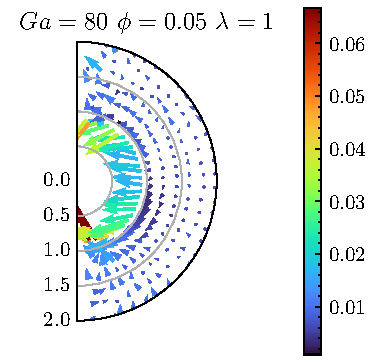
\includegraphics[width=0.3\textwidth]{image/HOMOGENEOUS_final/Dist/F_rel_l_1_Ga_80_PHI_5}
        \caption{Averaged force vector applied on the droplet present at the origin, conditioned on the presence of a nearest neighbor.
        The radial distance is made dimensionless by the droplets' diameter. 
        The color map represents the magnitude of the forces.}
        \label{fig:perspective_forces}
    \end{figure}
    On \ref{perspective_forces} we display our first result regarding the interaction forces statistic. 
    According to \citet{zhang2021ensemble} one remark \ref{fig:perspective_forces} is exactly a visual representation of teh particle-fluid-particle stress. 
    \item Altrough the most relevent closure of the continuous phase equations have been treated in this PhD work (Reynolds stress, drag force and stresslet), the closure terms of the disperse phase, specifically the particles center of mass velocity fluctuation $\pavg{\textbf{u}_\alpha'\textbf{u}_\alpha'}$, that is still need to be modeled. 
    Using a combination of Neast-Particle statistics and reflection method it is actually possible to derive an analytical model in the Stokes and Dilute regime. 
    The methodology is very similar to what is done in \ref{chap:pseudoturbulence}. 
    The first results gives, 
    \begin{equation*}
        \pavg{\textbf{u}_\alpha'\textbf{u}_\alpha'}
        % = 
        % n_p[\textbf{x},t]
        % \int_{\mathbb{R}^3}
        % (\textbf{v}^\text{nst}_p
        % \textbf{v}^\text{nst}_p)[\textbf{x},\textbf{y},t]
        % P_\text{nst}[\textbf{y}|\textbf{x},t]
        % d\textbf{y}
        = 
        C_1[\textbf{u}_{fp}\textbf{u}_{fp} - \frac{1}{3}(\textbf{u}_{fp}\cdot \textbf{u}_{fp})\bm\delta] 
        + C_2(\textbf{u}_{fp}\cdot \textbf{u}_{fp})\bm\delta
    \end{equation*}
    \begin{align}
      C_1 = \frac{1}{960}\left(\frac{2+3\lambda}{\lambda+1}\right)^2 \left[
        108\Gamma(1/3)
        - 80\Gamma (4/3)
        +15\Gamma(7/3)
      \right]\phi^{2/3}\\
      C_2 = \frac{1}{576}\left(
        \frac{2+3\lambda}{\lambda+1}\right)^2 \left[
        24\Gamma(1/3)
        - 16\Gamma (4/3)
        +3\Gamma(7/3)
      \right]\phi^{2/3}
    \end{align}
    For solid particle ($\lambda=\infty$) we find $\sqrt{k_p} = 1.52\phi^{1/3}$, while the experimental results reported in \citet{guazzelli2011fluctuations} suggest $\sqrt{k_p} = 2\phi^{1/3}$ and $3\phi^{1/3}$ which is higher. 
    First results are promising, more work on this topic is clearly needed.
    This study might lead to solve the famous Carlfish-Luke paradox \citet{caflisch1985variance}. 
\end{enumerate}

\paragraph*{Might be necessary}
Then there is points that might be relevant for this work, however at this stage it is hard to estimate the acctual needs.
\begin{enumerate}
    \item Another point of major importance not presented in this manuscript is the study of particle-fluid-particle stress, or long range interaction stress. 
    According to \cite{Lhuillier_2009,nott2011suspension,zhang2021ensemble} the drag force term can be expressed as a pure drag force term (that is the closure provided in \ref{chap:mono-disperse}) plus the divergence of a stress, the so-called particle-fluid-particle stress. 
    The latter stress would be responsible (among other term), for particle migration phenomenon.  
    At this stage it is hard to estimate if this stress is more or less important than the center of mass velocity variance, anyhow studies remain to be done to determine this contribution. 
    \item More generally up to know we considered homogeneous rising emulsion, however it might be relevant to take in account gradient of particle concentration in all of our closure terms. 
    The recent study of \citet{wang2024effect} started to include the gradient of volume fraction in the drag force closure. 
    \item Although we studied the first moment of hydrodynamic at low but finite inertial effect, it seems important to develop a model that is valid at higher Reynolds number and volume fraction since it seems that it could have a predominant effect on the stress in dense regime. 
    This can be carried out using the same DNS as presented in this work. 
    \item The study of the second moment of the hydrodynamic forces seems absent of the literature, while in our case where the flotation effects are dominant it remains important. 
    \item Finally, all of our closure terms consider a steady-state situation, meaning that we neglect the contribution from dispersed or continuous phase acceleration in our closure. 
    For the drag force this would correspond to added mass effect and that is known to be important. 
    For the other moment of forces this kind of contribution must be determined as well in terms of the unknowns of the problem. 
\end{enumerate}
These points mainly concerns the needs in closure models, a more general and thecnical conclusion on the closure model of the momentum equaitons is provided in \ref{ap:momentum_formulation} 


\paragraph*{Ideas of reaserch topics}
Now we would like to mention some ideas that seem pertinent for the modeling of multi-phase flow. 
\begin{enumerate}
    \item PR-DNS can be quite expansive to develop closure. 
    Thus, one might consider solving the single-particle conditioned averaged equations to produce closure.  
    Indeed, as demonstrated by \citet{hinch1977averaged} by considering closure within those equaitons one is able to derive more completet closure term, such as the second oreder correction of the equivalent stress and sedimentation velocity in this case. 
    Nevertheless, this approch is theoritically difficult, limiting the number of problem that can be traeated. 
    Solving this equation using numerical approach would enable us to consider more complicated scenario. 
    For example we could prescribe a given pair-distribution in the equations leading to closure model in terms of that pair-distribution; that could represent mean gradient of volume fraction, layers in the microstructure etc\ldots. 
    \item A second idea that seem relevant, is the use of the volume-averaged momentum bulk-equations presented in \ref{chap:daniel15} instead of the continuous phase averaged equation commonly used to describe the continuous phase momentum.
    This is interesting since this equations has the same form as classical N-S equaitons enabling us to use the single phase NS solver to describe the bulk-phase. 
    A set of equations for the dispersed phase is then added following the usual procedure. 
    A summary of this approach is given in \ref{ap:momentum_formulation}. 
\end{enumerate}
